\chapter{Implementation}

\section{Project Design}
// Update these pictures
\begin{figure}[!htbp]
    \label{fig:project-design}
    Use Case 1
    \begin{center}
    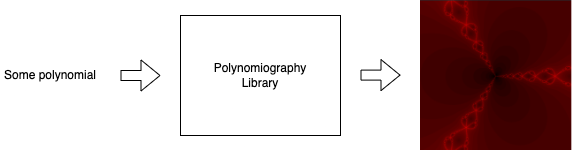
\includegraphics[width=0.8\textwidth]{Imgs/fig2.png}    
    \end{center}
    Use Case 2
    \begin{center}
    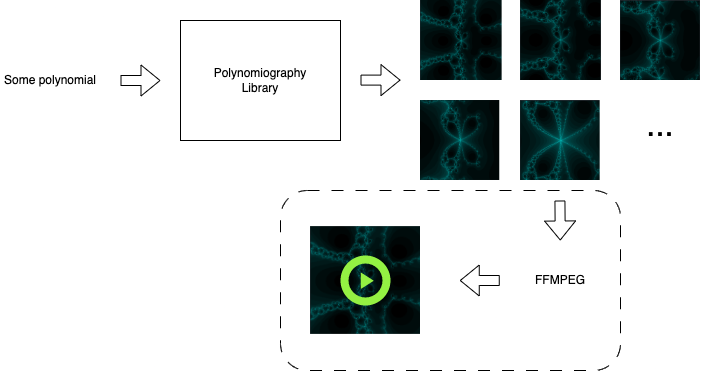
\includegraphics[width=0.8\textwidth]{Imgs/fig3.png}  
    \end{center}
    Use Case 3
    \begin{center}
    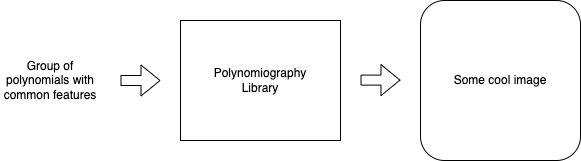
\includegraphics[width=0.8\textwidth]{Imgs/fig6.png}
    \caption{High Level Project Design}
    \end{center}
\end{figure}

\section{Implementation Details}

\subsection{Canvas $\iff$ Complex Plane}

\begin{figure}[!htbp]
    \centering
    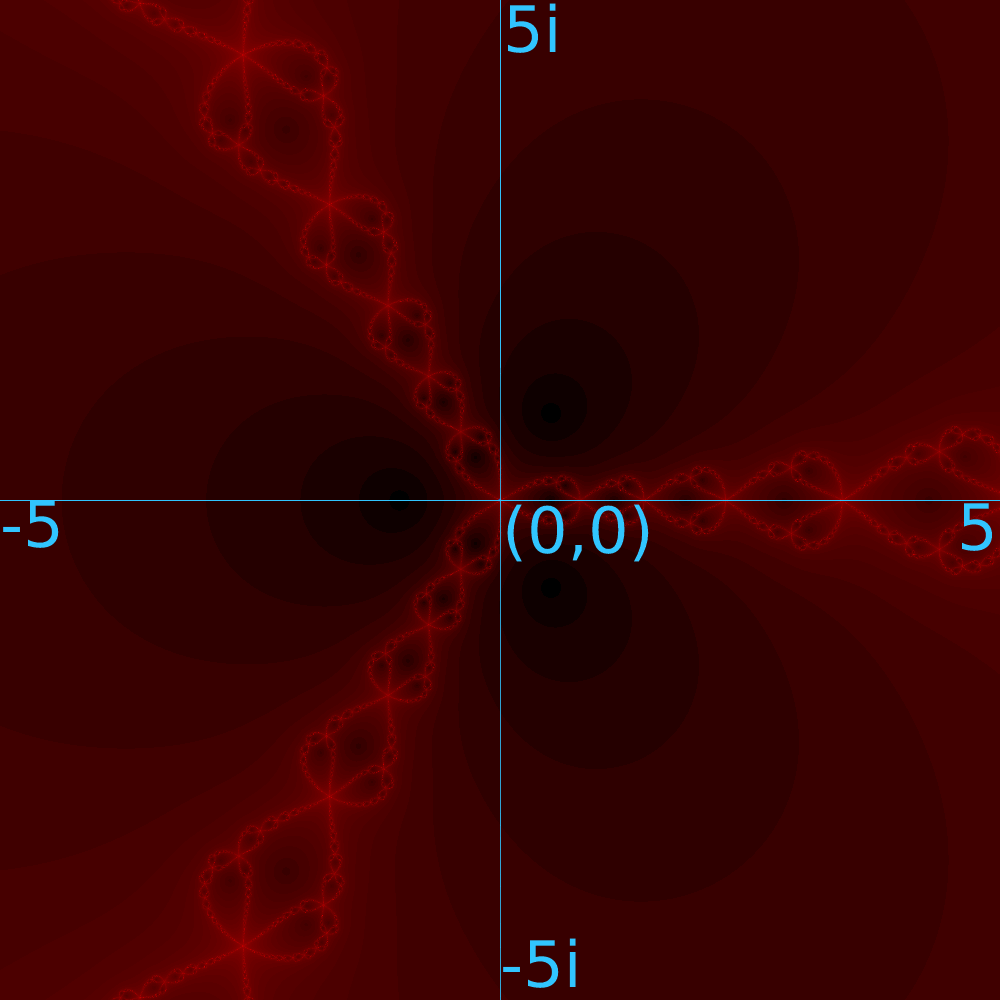
\includegraphics[width=0.6\textwidth]{Imgs/fig4.png}
    \caption{Complex plane on canvas}
    \label{fig:canvas-complex-plane}
\end{figure}

\subsection{Visualization of Iterative Root Finding Methods}

// Elaborate\\
-   For each pixel find the corresponding complex number\\
-   Start the iterative method with the corresponding number\\
-   Get the total iteration count until it converges\\
-   Assign a color to this pixel with respect to iteration count\\

\subsection{Visualization of Roots of Polynomial Rings Over Finite Fields}

// Elaborate\\
-   Compute the roots for each polynomial in finite field \\
-   Iterate over each root, find the corresponding pixel from the complex number\\
-   Increase the color on that pixel\\

\section{Usage}

For detailed usage see \hyperref[Appendix 1]{API Documentation}
